\documentclass[letterpaper, 10 pt, conference]{IEEEtran}
\IEEEoverridecommandlockouts
\overrideIEEEmargins

% -------------------------------------------------------------------------------------
% PACKAGES
% -------------------------------------------------------------------------------------
% *** STYLE PACKAGES ***
\usepackage{ieeehref}
\usepackage{ieeecref}

% *** CITATION PACKAGES ***
\usepackage{cite}

% *** GRAPHICS RELATED PACKAGES ***
\usepackage[dvips]{graphicx}
\usepackage{subfigure}

% *** MATH PACKAGES ***
\usepackage[cmex10]{amsmath}
\usepackage{amssymb}

% *** SPECIALIZED LIST PACKAGES ***
\usepackage{color}
%\usepackage{enumerate}
%\usepackage{algorithm,algorithmic

% *** PDF, URL AND HYPERLINK PACKAGES ***
%\usepackage{url}

% Adding a typewritten header -------------
\usepackage{fancyhdr}
\renewcommand{\headrulewidth}{0pt}
\chead{\tt{IEEE Int.Conf.on Tech.for Practical Robot Applications (TEPRA'13), 2013}}
% NOTE THAT IN ORDER TO USE THIS, you still need to add the following two lines
% After: \begin{document}
% \pagestyle{empty}
% \thispagestyle{fancyplain}
% --------------------------------------

% correct bad hyphenation here
%\hyphenation{op-tical net-works semi-conduc-tor}

% -------------------------------------------------------------------------------------
% MACROS
% -------------------------------------------------------------------------------------
\providecommand{\T}[0]{\textsf{T}} % Transpose
\providecommand{\abs}[1]{\lvert#1\rvert} % Absolute value
\providecommand{\norm}[1]{\lVert#1\rVert} % Norm
\renewcommand{\vector}[2]{[#1_1,\ldots,#1_{#2}]} % Vector
\newcommand{\argmin}{\operatornamewithlimits{argmin}} % Minimum argument
\newcommand{\argmax}{\operatornamewithlimits{argmax}} % Maximum argument
\providecommand{\N}{\mathbb{N}} % Natural Numbers
\providecommand{\Z}{\mathbb{Z}} % Integers Numbers
\providecommand{\R}{\mathbb{R}} % Real Numbers
\renewcommand{\Im}{\mathcal{R}} % Range Space
\providecommand{\Ker}{\mathcal{N}} % Null Space
\providecommand{\note}{\textcolor{red}} % Notes
\providecommand{\atan}{\mathrm{atan2}} % atan2 in normal font

\makeatletter
\let\@afterindenttrue\@afterindentfalse
\@afterindentfalse
\makeatother

% -------------------------------------------------------------------------------------
% THEOREMS
% -------------------------------------------------------------------------------------
% \newtheorem{thm}{Theorem}

% -------------------------------------------------------------------------------------
% BEGIN DOCUMENT
% -------------------------------------------------------------------------------------
\begin{document}
\bibliographystyle{ieeetr}
\pagestyle{empty}
\thispagestyle{fancyplain}


% -------------------------------------------------------------------------------------
% TITLE AND AUTHORS
% -------------------------------------------------------------------------------------
\title{\LARGE \bf
Humanoid Robot Teleoperation for Tasks with Power Tools
}

\author{Rowland O'Flaherty$^{\dagger}$, Peter Vieira$^{\dagger}$, M.X. Grey$^{\dagger}$, \\ Paul Oh$^{\ddagger}$, Aaron Bobick$^{\dagger}$, Magnus Egerstedt$^{\dagger}$, and Mike Stilman$^{\dagger}$%
\thanks{$^\dagger$Authors are affiliated with Georgia Institute of Technology, Atlanta, GA, 30332, USA. {\tt\small \{rowland.oflaherty, plvieira, mxgrey, magnus\}@gatech.edu} and {\tt\small \{afb,mstilman\}@cc.gatech.edu}.}%
\thanks{$^\ddagger$Author is affiliated with Drexel University, Philadelphia, PA, 19104, USA. {\tt\small paul@coe.drexel.edu}.}%
}

% Make the title area
\maketitle
\pagestyle{plain}
\thispagestyle{fancyplain}

% -------------------------------------------------------------------------------------
% ABSTRACT
% -------------------------------------------------------------------------------------
\begin{abstract}
This paper presents the implementation of inverse kinematics to achieve teleoperation of a physical humanoid robot platform. The humanoid platform will be used to compete in the DARPA Robot Challenge, which requires autonomous execution of various search and rescue tasks, such as cutting through walls, which is a very practical application to robotics. Using a closed-form kinematic solution and a basic feedback controller, our objective of executing simple tasks is realized via teleoperation. Joint limits and singularities are accounted for using the different cases in the kinematic solution; and a decision method is implemented to determine how to position the end-effector when the goal is outside the feasible workspace. 
\end{abstract}

% -------------------------------------------------------------------------------------
% INTRODUCTION
% -------------------------------------------------------------------------------------
\section{Introduction} \label{sec:introduction}
In this paper we present, analyze and evaluate the teleoperation of a humanoid robot platform using a feedback controller and the inverse kinematics of the limbs. The particular humanoid platform that is used in this work is the HUBO$\,$2+ platform (Hubo). Teleoperation of the arms is performed using a Polhemus FASTRAK motion tracking system for tasks in order to provide preliminary proof of concept of methods that will later be used to execute tasks autonomously in search and rescue missions. Hubo has six degrees of freedom (DOF) in each arm and leg, which is the minimum number of DOF required to control the three position and orientation variables. We have developed algorithms to control Hubo in the end-effector workspace via teleoperation using a closed-form kinematic solution and a basic feedback controller in order to execute simple tasks, such as using a rotary tool to cut out holes in a cardboard wall, see \cref{fig:Top-image}.

Ali et. al. presented a closed-form solution for the inverse kinematics (IK) of the limbs of the HUBO$\,$2+ robot platform \cite{Ali:2010wm}. They used a reverse decoupling mechanism method by viewing the kinematic chain of a limb in reverse order and decoupling the position and orientation. The authors then used the inverse transform method to compute eight possible solutions, with the correct solution selected based on joint limits and constraints. In working through their solution, discrepancies were found in the calculations. We corrected the errors and solved for the IK of all four limbs for our HUBO\,2+ humanoid robot. 

There has been significant recent work on teleoperation of humanoid robots, such as \cite{stilman:ke} and \cite{Miller:el}, but few of them use tools to perform practical tasks. There is research being conducted on robots using tools, for instance \cite{Ambrose:2000gx} and \cite{Hasunuma:uk}, but these focus more on the design of robots for using tools, rather than the acutal utilization of tools to perform specific tasks. Our teleoperation of the HUBO$\,$2+ robot goes beyond design into the realm of performing useful tasks.  

\begin{figure}[t]
  \centering
  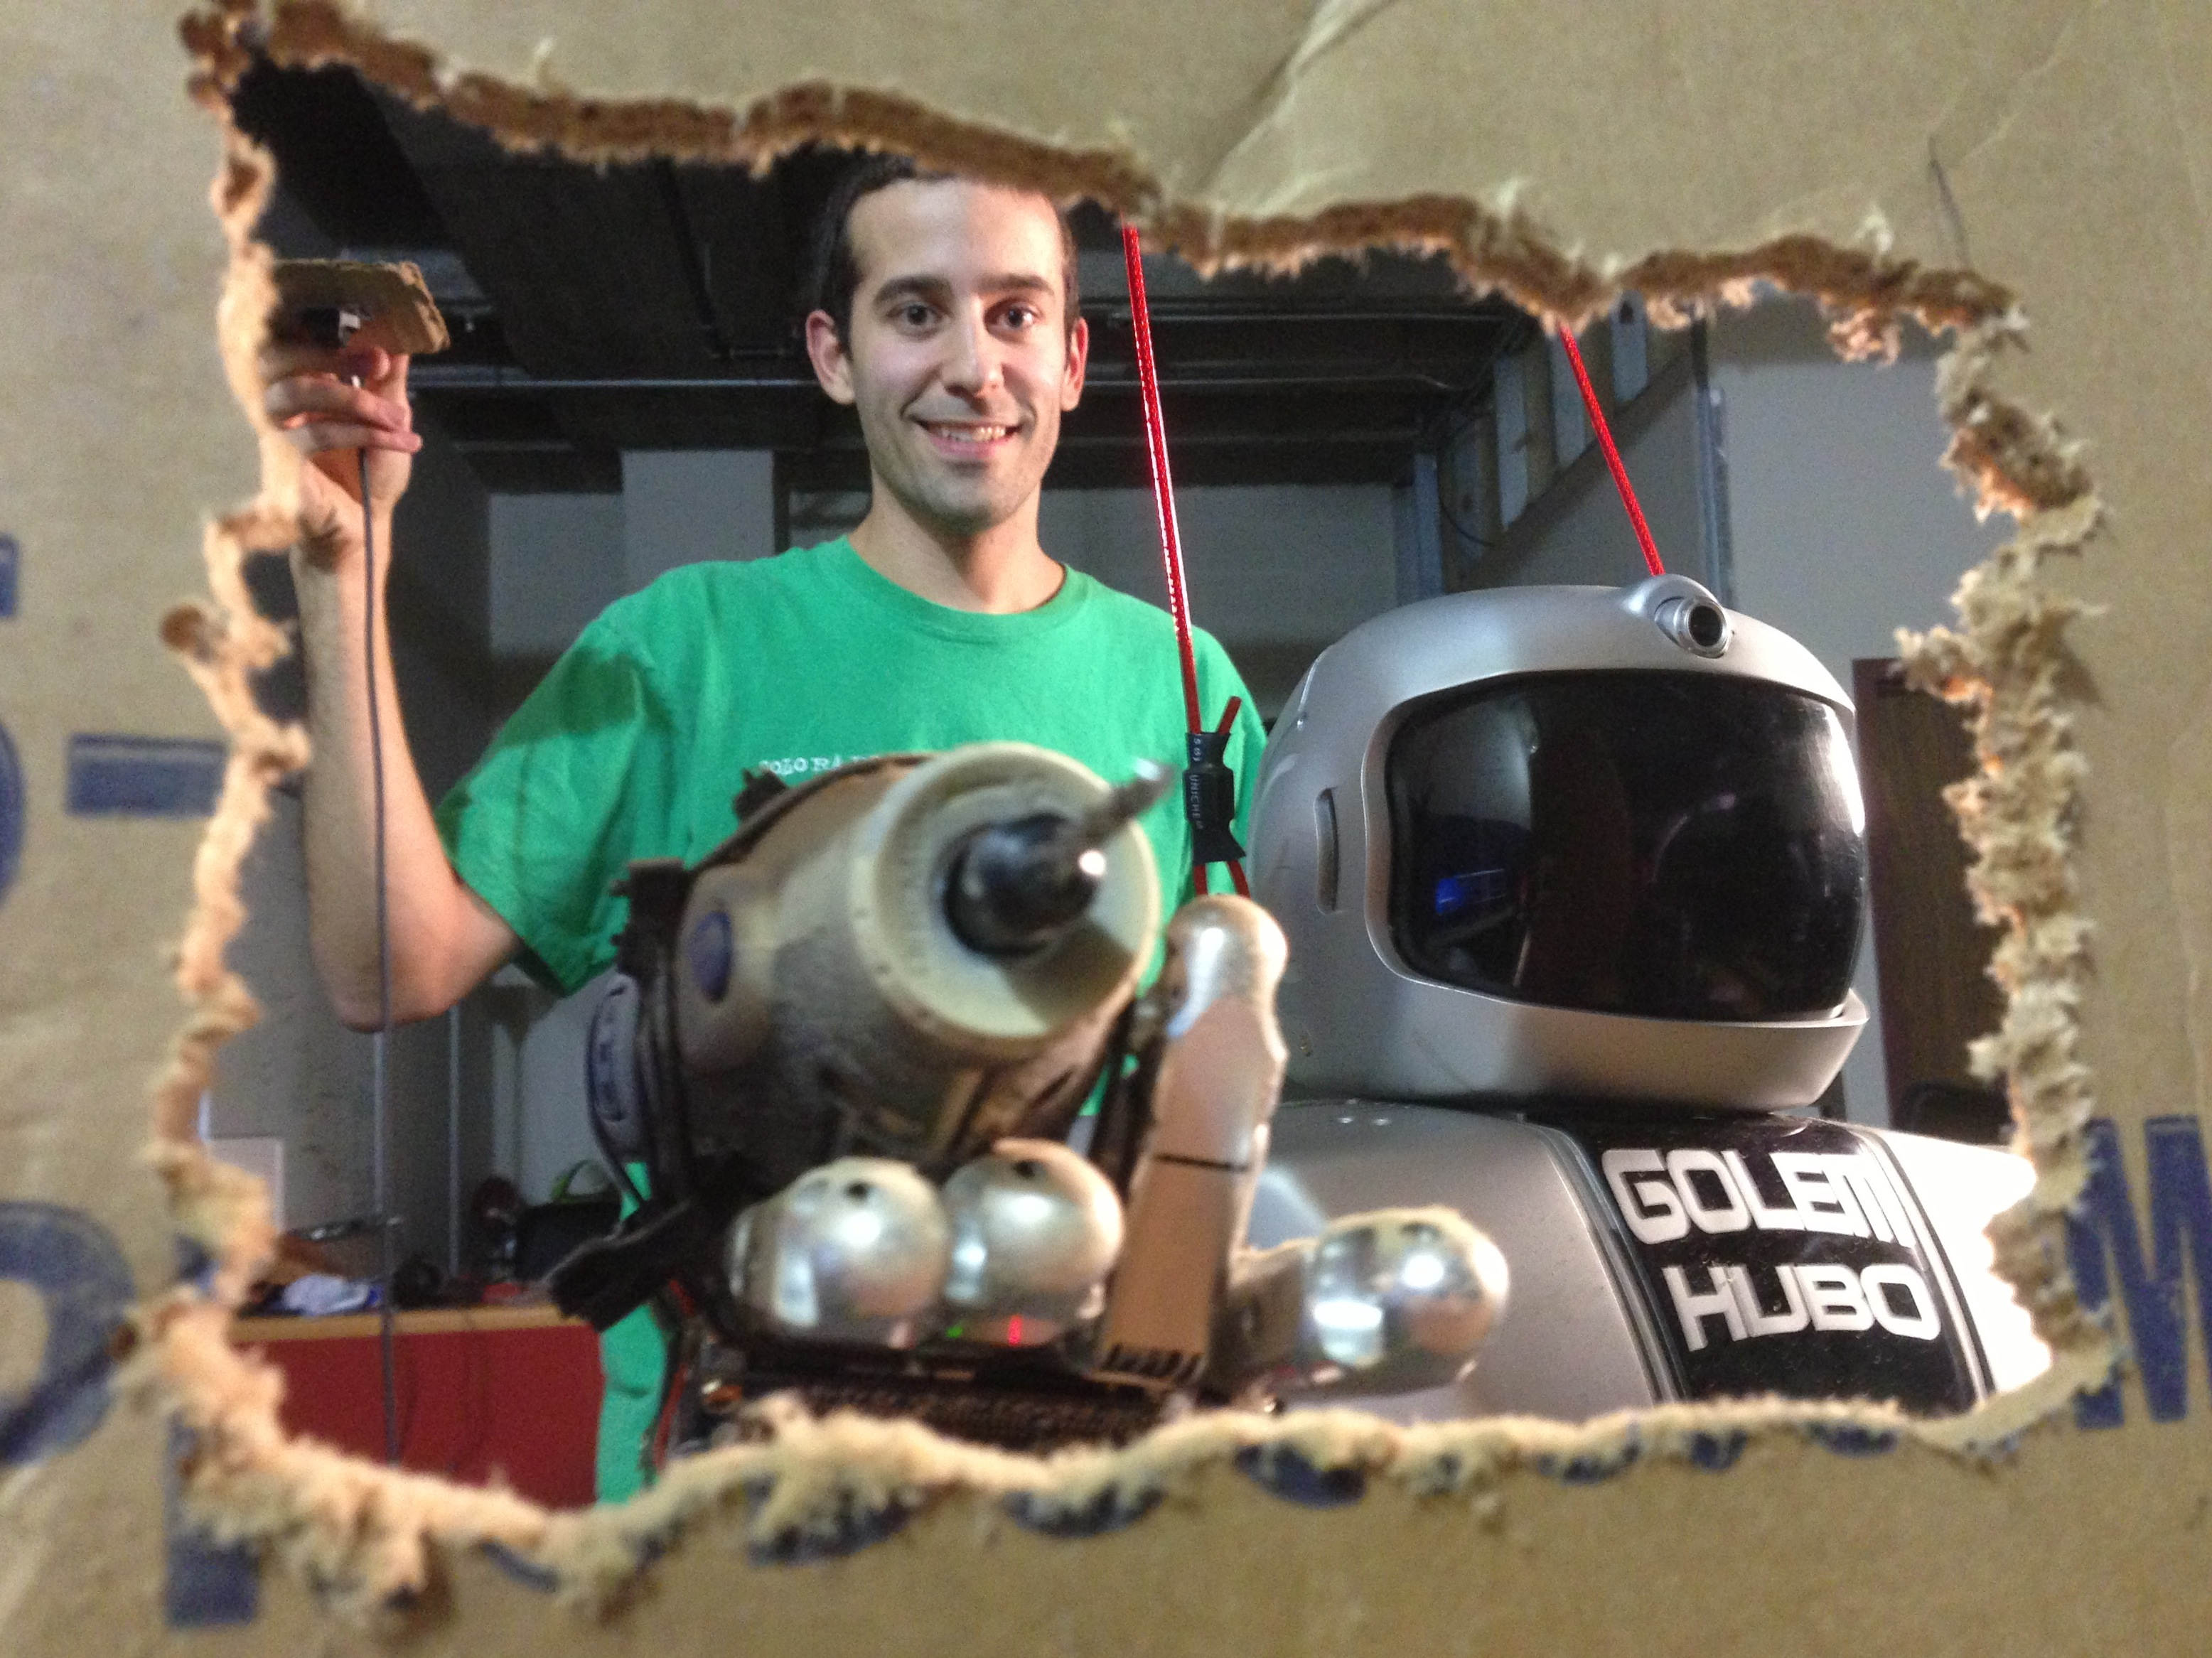
\includegraphics[width=0.4\textwidth]{figures/Top-image}
  \caption{Picture of Hubo and operator just after using telemanipulation to cut a rectangular hole out of a cardboard wall. }
  \label{fig:Top-image}
\end{figure}

% -------------------------------------------------------------------------------------
% HUBO GEOMETRY AND KINEMATICS
% -------------------------------------------------------------------------------------
\section{Hubo Geometry and Kinematics} \label{sec:huboGeoKinematics}
In order to control Hubo using workspace control via teleoperation both forward and inverse kinematic solutions are required. The solution to this problem involves solving for the joint angles given a desired position and orientation while accounting for singularities, joint limits and feasible workspace issues.

The kinematic structure of the right and left arm of Hubo are identical, therefore they have the same joint coordinate frames, as well as the same Denavit-Hartenberg (DH) parameters. The only difference is the offset direction from the base frame at the neck. The left and right leg also have the same kinematic structure as each other, thus their solutions differ only in the offset from the base frame. We first go through the solution for the IK of the arms, and then the legs. The joint coordinate frames are shown in \cref{fig:huboCoordinates} and the length of each link is shown in \cref{tbl:linkLengths}. The DH parameters (using the standard convention) for the arms and legs are shown in \cref{tbl:armDH} and \cref{tbl:legDH}, respectively. 

\begin{figure}[h]
  \centering
  \includegraphics[width=0.3\textwidth]{figures/Hubo-Coordinates.pdf}
  \caption{Hubo coordinate frames}
  \label{fig:huboCoordinates}
\end{figure}

\begin{table}[h] 
    \centering
    \caption{Link lengths of Hubo}
    \begin{tabular}{|c|c|} \hline
    \multicolumn{2}{|c|}{Lengths of arm links} \\ \hline
    	Link &  Length (mm) \\ \hline
		$l_{A1}$ & 211 \\ \hline %211
    	$l_{A2}$ & 182 \\ \hline %179.14
   	    $l_{A3}$ & 164 \\ \hline %164.0
    	$l_{A4}$ & 121 \\ \hline %120.6
    	$l_{E}$ & 100 \\ \hline %177.8
    \end{tabular}
    \begin{tabular}{|c|c|} \hline
    \multicolumn{2}{|c|}{Lengths of leg links} \\ \hline
    	Link &  Length (mm) \\ \hline
    	$l_{T}$ & 187 \\ \hline %186.5
    	$l_{L1}$ & 88 \\ \hline %88.43 from hubo+ urdf
    	$l_{L2}$ & 167 \\ \hline %167.3 from hubo+ urdf
    	$l_{L3}$ & 280 \\ \hline %280.0 from hubo+ urdf
    	$l_{L4}$ & 280 \\ \hline %279.9 from hubo+ urdf
    	$l_{L5}$ & 95 \\ \hline %94.97
    \end{tabular} \label{tbl:linkLengths}
\end{table}

\subsection{Forward Kinematic Solution for the Arm}
The forward kinematics problem is that of solving for the end-effector orientation and position given the joint angles. This is easily solved using the geometry of the robot which is specified in the DH parameters. The general homogeneous transformation from one link to the next given the DH parameters is represented in matrix form as:
\begin{equation}\label{eq:transformDHMatrix}\resizebox{.9\hsize}{!}{$
^{i-1}T_i = 
	\begin{bmatrix}
		\cos(\theta_i) & -\sin(\theta_i)\cos(\alpha_i) & \sin(\theta_i)\sin(\alpha_i) & \mathrm{a}_i\cos(\theta_i) \\%[0.3em]
    	\sin(\theta_i) & \cos(\theta_i)\cos(\alpha_i) & \mathrm{-}\cos(\theta_i)\sin(\alpha_i) & \mathrm{a}_i\sin(\theta_i) \\%[0.3em]
    	0 & \sin(\alpha_i) & \cos(\alpha_i) & \mathrm{d}_i \\%[0.3em]
  		0 & 0 & 0 & 1
	\end{bmatrix}$}.
\end{equation}
where ${^{i-1}T_i}$ is the transformation from coordinate frame $i-1$ to frame $i$. The base frame for the arm is at the neck, and its tranformation to the first shoulder joint is 
\begin{align}\label{eq:neckMatrix}
^NT_0= \begin{bmatrix}
	1 & 0 & 0 & 0 \\
	0 & 0 & 1 & l_{A1} \\
	0 &-1 & 0 & 0 \\
	0 & 0 & 0 & 1
\end{bmatrix}.
\end{align}
An additional transformation $^6T_E$ is used for the transformation from the hand to the end-effector\footnote{This transformation is defined for a drill end-effector in the \cref{sec:implementation}.}.
In order to calculate the forward kinematics (FK) the six transformation matrices from each joint are pre-multiplied to obtain the position and orientation of the end-effector relavtive to the shoulder. We define the transformation from the shoulder to the hand as
\begin{align} \label{eq:shoulderToHandTransform}
^0T_6 &=\:^0T_1\:^1T_2\:^2T_3\:^3T_4\:^4T_5\:^5T_6.
\end{align}
Thus when solving for the forward kinematics $^0T_6$ must be pre-multiplied by $^NT_0$ and post-multiplied by $^6T_E$. Therefore, the FK is calculated as 
\begin{align} \label{eq:armFK}
^NT_E &=\:^NT_0\:^0T_6\:^6T_E.
\end{align}

\begin{table}[h]
    \centering
    \caption{DH parameters of the arms}
    \begin{tabular}{|c|c|c|c|c|} \hline
    \multicolumn{5}{|c|}{Right arm DH parameters} \\ \hline
    Coord. Frame i &  $\theta_i$              & $\alpha_i$  & $a_i$ & $d_i$ \\ \hline
          1 &  $\theta_1 + \pi/2$  & $\pi/2$  & 0     & 0 \\ \hline
    	  2 &  $\theta_2 - \pi/2$ & $\pi/2$  & 0     & 0 \\ \hline
   	  3 &  $\theta_3 + \pi/2$  & $-\pi/2$ & 0     & $-l_{A2}$ \\ \hline
    	  4 &  $\theta_4$              & $\pi/2$  & 0     & 0 \\ \hline
    	  5 &  $\theta_5$              & $-\pi/2$ & 0     & $-l_{A3}$ \\ \hline
    	  6 &  $\theta_6 + \pi/2$  & $0$   & $l_{A4}$ & 0 \\ \hline
    \end{tabular} \label{tbl:armDH}
\end{table}

\subsection{Inverse Kinematic Solution for the Right Arm}
The inverse kinematics problem is how to solve for the joint angles given the end-effector orientation and location, specified as $^NT_E$. This is a much harder problem because there are multiple solutions. When solving the inverse kinematics of a manipulator, Pieper \cite{Peiper:1968wi} indicates that a closed-form solution exists if three consecutive joint axes of the manipulator are parallel to one another, or intersect at a single point. The three shoulder joint axes on the Hubo intersect at a single point for the arm and the three hip joints intersect at a single point for the leg, therefore a closed-form kinematic solution exists for each. 

We will solve the IK problem from the shoulder to the hand by using the transformation $^0T_6$. This is obtained by pre-multiplying $^NT_E$ by $^0T_N$ and post-multiplying by $^ET_6$. Let us write the $^0T_6$ obtained from $^NT_E$ as
\begin{align} \label{eq:totalTransformExpand}
^0T_6 &= \begin{bmatrix}
	\mathrm{x}_6 & \mathrm{y}_6 & \mathrm{z}_6 & \mathrm{p}_6 \\
	0   & 0   & 0   & 1
\end{bmatrix}
= \begin{bmatrix}
	\mathrm{n} & \mathrm{s} & \mathrm{a} & \mathrm{p} \\
	0 & 0 & 0 & 1
\end{bmatrix},
\end{align}
where $\textrm{x}_6$, $\textrm{y}_6$, and $\textrm{z}_6$ are the unit vectors along the principal axes of the hand frame and $\textrm{p}_6$ is the position vector describing the location of the hand relative to the shoulder. These three unit vectors describe the orientation of the hand coordinate frame relative the the shoulder coordinate frame. The vectors $n$, $s$, $a$, and $p$ represent the normal vector, sliding vector, approach vector, and position vector of the hand, respectively \cite{Fu:1987uu}.

Using this knowledge, the arm can be viewed in reverse so that the last three joints make up the shoulder, thus the position and orientation of the shoulder frame can be described relative to the hand frame. This new position vector, $p^\prime$, is only a function of $\theta_4$, $\theta_5$ and $\theta_6$, and thus decouples the arm into position and orientation components. The IK-problem is solved in this reverse method by taking the inverse of both sides of \eqref{eq:totalTransformExpand}.
\begin{align}\label{eq:inverseTotalTransform}
^0T_6\,^\prime = \,^6T_0 = (^0T_6)^{-1} = 
	\begin{bmatrix}
    	\mathrm{n^\prime} & \mathrm{s^\prime} & \mathrm{a^\prime} & \mathrm{p^\prime} \\
    	0 & 0 & 0 & 1
	\end{bmatrix}
\end{align}
As in \cite{Ali:2010wm}, we solved for the joint angles using the reverse method. The joint solutions are given below. The details on how these solutions were derived are in the following tech report \cite{O'Flaherty:2013inverseIK}.

First, the three lower joint angles of $A_4$, $A_5$ and $A_6$ are solved for and then the upper joint angles of $A_1$, $A_2$ and $A_3$ are solved for. The solutions are as follows:\footnote{The sine and cosine of an angle $\alpha$ is abbreviated $S_\alpha$ and $C_\alpha$, respectively}~\footnote{$wrapToPi(\alpha)$ wraps the angle $\alpha$ to the interval between $-\pi$ and $\pi$.}

\begin{align}
  \theta_4 &= \atan(\pm real(\sqrt{1-C_4^2}), C_4), \nonumber \\
  C_4 &= \frac{(p_x^\prime + l_{A4})^2 + p_y^\prime\,^2 + p_z^\prime\,^2 - l_{A2}^2 - l_{A3}^3}{2l_{A}2l_{A3}}; \nonumber \\
  \theta_5 &= \atan(S_5, \pm real(\sqrt{1-S_5^2})),~~S_5 = p_z^\prime/(S_4l_{A2}); \nonumber \\
  \theta_6 &= wrapToPi(\atan(S_4C_5l_{A2}, -C_4l_{A2} - l_{A3}) - \psi), \nonumber \\
  \psi &= \atan (p_y^\prime, p_x^\prime + l_{A4}); \nonumber \\
  \theta_2 &= \atan(S_2, \pm real(\sqrt{1-S_2^2})), \nonumber \\
  S_2 &= a_x^\prime(C_4C_6 - C_5S_4S_6) - a_y^\prime(C_4S_6 + C_5C_6S_4) \nonumber \\
  &\quad - a_z^\prime S_4S_5; \nonumber
\end{align}
\begin{align}
  \theta_3 &= \atan(S_3, C_3), \nonumber \\
  S_3 &= g_{313} = - a_x^\prime(C_6S_4 + C_4C_5S_6) + a_y^\prime(S_4S_6 - C_4C_5C_6) \nonumber \\
  &\quad\quad\quad\quad - a_z^\prime C_4S_5, \nonumber \\
  C_3 &= g_{333} = - a_x^\prime S_5S_6 - a_y^\prime C_6S_5 + a_z^\prime C_5; \nonumber \\
  \theta_1 &= \atan(S_1, C_1), \nonumber \\
  S_1 &= -n_x^\prime(C_4C_6 - C_5S_4S_6) + n_y^\prime(C_4S_6 + C_5C_6S_4) + \nonumber \\
  &\:\:\:\:\:\:\:\:\: n_z^\prime S_4S_5, \nonumber \\
  C_1 &= s_x^\prime(C_4C_6 - C_5S_4S_6) - s_y^\prime(C_4S_6 + C_5C_6S_4) - \nonumber \\
  &\:\:\:\:\:\: s_z^\prime S_4S_5. \nonumber
\end{align}

There are two solutions for $\theta_2$, $\theta_4$, and $\theta_5$, which generate eight total solutions to the arm IK. When the goal position is outside the feasible workspace of the limb, the joint solutions will have imaginary parts. To deal with this, we take only the real part, which in turn gives the solution that is closest to the desired position. Furthermore there are five cases that result in singularities, and details of the solution methods can be viewed in \cite{Ali:2010wm}. The following are our final equations for each case.

\subsubsection{Case 1 (elbow singularity)} When $\theta_4$ = 0, joints $\theta_3$ and $\theta_5$ are collinear, thus an infinite number of solutions exist to orient the end-effector in the desired orientation. We set $\theta_3$ to its previous value and then the difference between the $\theta_5$ and $\theta_3$, $\theta_T$, is set to the desired orientation by solving the equation,
\begin{align}
&	\theta_T = \atan(-C_6a_y^\prime - S_6a_x^\prime, a_z^\prime) \nonumber \\
&	\mathrm{if}\: C_2 < 0,\:\mathrm{ then~}\: wrapToPi(\theta_T = \theta_T + \pi) \nonumber \\
&	\theta_5 = wrapToPi(\theta_T - \theta_3). \nonumber
\end{align}

\subsubsection{Case 2 (shoulder singularity)} When $\theta_2$ = $\pi/2$ (for the left arm) or $-\pi/2$ (for the right arm) joints $\theta_1$ and $\theta_3$ are collinear. The same approach as above is taken, resulting in the difference equation,
\begin{align}
&	\theta_T = \atan(S_6s_y^\prime - C_6s_x^\prime, S_6n_y^\prime - C_6n_x^\prime) \nonumber \\
&	\mathrm{if}\: S_4 < 0, \theta_T = \theta_T + \pi \nonumber \\
&	\text{Left \:Arm:  } \theta_1 = wrapToPi(\theta_T + \theta_3) \nonumber \\
&	\text{Right \:Arm:  } \theta_1 = wrapToPi(\theta_T - \theta_3). \nonumber
\end{align}

\subsubsection{Case 3 (left arm singularity)} When $\theta_4$ = 0 and $\theta_2$ = $\pi/2$ (for the left arm) or $-\pi/2$ (for the right arm) joints $\theta_1$, $\theta_3$ and $\theta_5$ are collinear. The same approach as above is taken, resulting in the difference equations,
\begin{align}
&	\text{Left \:Arm:  } \theta_T = \atan(n_z^\prime, -s_z^\prime) \nonumber \\
&	\theta_5 = wrapToPi(\theta_1 - \theta_3 - \theta_T),\nonumber \\
&	\text{Right \:Arm: } \theta_T = \atan(-n_z^\prime, s_z^\prime) \nonumber \\
&	\theta_5 = wrapToPi(\theta_T - \theta_1 - \theta_3).
\end{align}

After solving for the joint angles, eight solutions exist. To select the correct solution, joint constraints are considered. Finally, when solving for the inverse kinematics the inverse of the neck-to-shoulder transformation matrix, $^0T_N$, must first be pre-multiplied and the inverse of the hand transformation matrix, $^ET_6$, must be post-multiplied in order to compute the IK using the DH parameters.

\subsection{Forward Kinematic Solution for the Leg}
As with the arm the forward kinematics of the leg, $^NT_F$, are straighted forward once the DH parameters are derived. The DH parameters for the right leg are shown in \cref{tbl:legDH} and again \eqref{eq:transformDHMatrix} is used find the transformation between adjacent joint coordinate frames. The base frame for the leg is at the waist, and its tranformation to the first hip joint is,
\begin{align}\label{eq:hipTransformMatrix}
^NT_w= \begin{bmatrix}
	1 & 0 & 0 & 0 \\
	0 & 1 & 0 & 0 \\
	0 & 0 & 1 & -l_{L_T} \\
	0 & 0 & 0 & 1
\end{bmatrix}
{^WT_0} = \begin{bmatrix}
	0 & -1 & 0 & 0 \\
	1 & 0 & 0 & l_{L1} \\
	0 & 0 & 1 & -l_{L2} \\
	0 & 0 & 0 & 1
\end{bmatrix}.
\end{align}
We define the transformation from the hip to the foot as 
\begin{align} \label{eq:hipToFootTransform}
^0T_6 &=\:^0T_1\:^1T_2\:^2T_3\:^3T_4\:^4T_5\:^5T_6.
\end{align}
Thus when solving for the forward kinematics $^NT_F$ must be pre-multiplied by $^NT_W\,^WT_0$ and post-multiplied by $^6T_F$. Therefore, the FK is calculated as 
\begin{align} \label{eq:armFK}
^NT_F &=\:^NT_w\:^WT_0\:^0T_6\:^6T_F.
\end{align}

\begin{table}[h]
    \centering
     \caption{DH parameters of the legs}
    \begin{tabular}{|c|c|c|c|c|} \hline
    \multicolumn{5}{|c|}{Right leg DH parameters} \\ \hline
    Coord. Frame i &  $\theta_i$          & $\alpha_i$ & a$_i$ & d$_i$ \\ \hline
   	  1 &  $\theta_1$          & $\pi/2$    & 0     & 0\\ \hline
    	  2 &  $\theta_2 - \pi/2$  & $-\pi/2$   & 0     & 0 \\ \hline
   	  3 &  $\theta_3$          & 0          & $l_{L3}$ & 0 \\ \hline
   	  4 &  $\theta_4$          & 0          & $l_{L4}$ & 0 \\ \hline
    	  5 &  $\theta_5$          & $\pi/2$    & 0     & 0 \\ \hline
    	  6 &  $\theta_6$          & 0          & $l_{L5}$ & 0 \\ \hline
    \end{tabular} \label{tbl:legDH}
\end{table}

\subsection{Inverse Kinematic Solution for the Leg}
Similar to the IK for the arm the IK for the leg is solved from the hip to the foot by using the transformation $^0T_6$. This is obtained by pre-multiplying $^NT_F$ by $^0T_W\:^WT_N$ and post-multiplying by $^FT_6$. Let us write $^0T_6$ for the legs in the same way as for the arms in \eqref{eq:totalTransformExpand}.

As with the arm, the three hip joint axes in the leg on Hubo intersect at a single point, therefore a closed-form kinematic solution exists. Thus the procedure for solving the IK for legs is similar to the arms. As with the IK of the arm the details of deriving the solutions for the joint angles are given in the following tech report \cite{O'Flaherty:2013inverseIK}.

First, the three lower joint angles of $L_4$, $L_5$, and $L_6$ are solved for, and then the three upper joint angles of $L_1$, $L_2$, and $L_3$ are solved for. The solutions are as follows:
\begin{align}
  \theta_4 &= \atan(\pm real(\sqrt{1-C_4^2}), C_4), \nonumber \\
  C_4 &= \frac{(p_x^\prime + l_{L5})^2 + p_y^\prime\,^2 + p_z^\prime\,^2 - l_{L3}^2 - l_{L4}^3}{2l_{L3}l_{L4}}; \nonumber \\
  \theta_5 &= wrapToPi(\atan(-p_z^\prime, \pm real(\sqrt{(p_x^\prime + l_{L5})^2 + p_y^\prime\,^2}) \nonumber \\
  &\quad- \psi),  \nonumber \\
  \psi &= \atan(S_4l_{L3}, C_4l_{L3}+l_{L4}); \nonumber \\
  \theta_6 &= \atan(p_y^\prime, -p_x^\prime-l_{L5});  \nonumber
\end{align}
\begin{align}
  S_2 &= S_6a_x^\prime + C_6a_y^\prime,  \nonumber \\
  \theta_2 &= \atan(S_6a_x^\prime + C_6a_y^\prime, \pm real(\sqrt{1 - (S_6a_x^\prime + C_6a_y^\prime)^2})); \nonumber \\
  \theta_1 &= \atan(S_6s_x^\prime + C_6s_y^\prime, S_6n_x^\prime + C_6n_y^\prime); \nonumber  \\
  C_2S_1 &= S_6s_x^\prime + C_6s_y^\prime, \nonumber \\
  C_2C_1 &= S_6n_x^\prime + C_6n_y^\prime; \nonumber \\
  \theta_3 &= wrapToPi(\theta_{345} - \theta_4 - \theta_5), \nonumber  \\
  \theta_{345} &= \atan(a_z^\prime, C_6a_x^\prime - S_6a_y^\prime). \nonumber
\end{align}
If $C_{45} l_{L3} + C_5 l_{L4} < 0$ then $\theta_6 = wrapToPi(\theta_6 + \pi)$.
If $C2 < 0$ then $\theta_1 = wrapToPi(\theta_1 + \pi)$.

We now have the inverse kinematic solution to the right leg. The above solution can be applied to the left leg by changing $+l_{L1}$ to $-l_{L1}$ in the base-to-hip transformation matrix in \eqref{eq:hipTransformMatrix}.

Like the arm there are two solutions for $\theta_2$, $\theta_4$ and $\theta_5$, which generate eight total solutions to the leg IK. As with the arm, if the goal position is outside the feasible workspace of the limb the joint solutions will have imaginary parts and only the real part is used.

\subsection{Choosing Joint Solution}
For the inverse kinematics of each of the arms and the legs there are eight joint solutions. The sum of squared joint values is the primary metric that is used in picking one of the eight solutions. Choosing the solution that minimizes this metric is the solution that is ``closest'' to the zero position of the joints. This works well if at least one of the solutions has all of its joints values within the joint limits (\cref{tbl:jointLimits}).

If none of the solutions have all the joint values within the limits then there is no solution that satisfies the desired pose (orientation and location). To get the end-effector to a position as close as possible to the desired position the joint values in all the solutions are capped at the closest joint limit value. Each of the solutions are then given to the FK to calculate the end-effector location with the capped joint values. The solution that gets the end-effector position the closest to the desired position is used. If none of the joint solutions get the end-effector within 5 cm of the desired position then the previous joint values are used.

\begin{table}[h]
    \centering
    \caption{Joint limits of the arms and legs}
    \begin{tabular}{|c|c|c|c|c||c|c|c|c|} \hline
    \ & \multicolumn{4}{|c||}{Arms} & \multicolumn{4}{|c|}{Legs} \\ \hline
    Joint & \multicolumn{2}{|c|}{Left} & \multicolumn{2}{|c||}{Right} & \multicolumn{2}{|c|}{Left} & \multicolumn{2}{|c|}{Right} \\ \hline
    i & min.  & max.  & min.  & max.  & min.  & max.  & min.  & max.  \\ \hline
    1 & -2.0 & 2.0 & -2.0 & 2.0 & 0 & 1.8 & -1.8 & 0 \\ \hline
    2 & -0.3 & 2.0 & -2.0 & 0.3 & 0 & 0.6 & -0.6 & 0 \\ \hline
    3 & -2.0 & 2.0 & -2 & 2.0 & -1.3 & 1.4 & -1.3 & 1.4 \\ \hline
    4 & -2.5 & 0 & -2.5 & 0 & 0 & 2.5 & 0 & 2.5 \\ \hline
    5 & -2.5 & 2.0 & -2.5 & 2 & -1.3 & 1.8 & -1.3 & 1.8 \\ \hline
    6 & -1.4 & 1.2 & -1.4 & 1.2 & -0.3 & 0.2 & -0.2 & 0.3 \\ \hline
    \end{tabular} \label{tbl:jointLimits}
\end{table}

% -------------------------------------------------------------------------------------
% Implementation
% -------------------------------------------------------------------------------------
\section{Implementation} \label{sec:implementation}
It takes more than just solving for the kinematics to actually have Hubo do something meaningful. In this section we describe various important considerations and algorithms that are needed to implement teleoperation on Hubo.

\subsection{Arm and Leg Inverse Kinematics} \label{sec:armAndLegIK}
The workspace of Hubo's arms is limited because the arms are short. To increase the vertical workspace of Hubo's arms, Hubo can use its legs to move its body up and down. Getting Hubo to move its end-effector to a desired location that requires its body to move up or down requires some form of inverse kinematics for all 12 joints of each arm and leg pair (left and right). To simplify this we assume that both hands will be working at the same height level and have developed an algorithm that uses the decouple inverse kinematics of the arms and the legs as described in \cref{sec:huboGeoKinematics}. To summarize this algorithm, Hubo keeps its hands at shoulder level and moves its body up and down with its legs. If a desired pose is below or above the points the body can be elevated to then the arms will move down or up from the fully lowered or raised body positions. 

The algorithm is as follows: (1) Get desired hand pose and extract height information; (2) Use leg IK to move the shoulder to as close as possible to desired height; (3) Use arm IK to move hand to desired hand pose.

\subsection{Control} \label{subsec:control}
Currently the motor control boards on Hubo only support position control. The gains for this position control are extremely high to deal with the external forces that the joints may encounter. Due to these high gains, giving arbitrary joint angles is not possible because the joint will move to the position in a violent manner. Therefore, a feedback controller algorithm is implemented using nominal maximum velocities and accelerations in order to achieve fluid, safe motion. This algorithm works by giving the motor control board for a given joint a trajectory to follow from its current position to the desired position that minimizes the jerk on the joints. This allows for the joint to reach the desired position by accelerating and decelerating in smooth fashion.

\subsection{Balancing} \label{subsec:balancing}
In order to achieve any of these task, balancing is a necessary reqirement. Four sensor values are used on Hubo to  achieve balancing. We obtain the angles, $\phi_x$ and $\phi_y$, about the x- and y-axes that the waist is at relative to the vertical z-axis from an inertial measurement unit (IMU) in his waist, and the moments, $M_x$ and $M_y$, about each ankle from the force/torque sensors in the feet. Often, when a humanoid plants its feet on the ground it creates a closed loop, which in turn can result in dangerously high torques if the feet happen to slide or shift relative to each other while still on the ground. This can cause the motors to draw extremely high current and potentially burn the motors out. One instance when this is an important consideration is when first placing the robot on the ground. If its feet are not both parallel to the ground, and the ankle motors are being used for balancing, then this phenomenon can arise. To avoid this problem we devised a method to even out the feet and then balance such that the ankle motors comply with the moments $M_x$ and $M_y$, but resist the IMU angles $\phi_x$ and $\phi_y$. We achieve this by setting the compliant term for the ankle angular velocities equal to a gain multiplied by the moment, and the resistive term equal to a gain multiplied by the IMU angle. Thus, the ankle angular velocities are
\begin{align}
\omega_{roll} = K_r\phi_x - K_cM_x, \\
\omega_{pitch} = K_r\phi_y - K_cM_y,
\end{align}
where $\omega_{roll}$ and $\omega_{pitch}$ are the angular velocities of the ankle roll and pitch joint motors, respectively, and $K_r$ and $K_c$ are the resistive and compliant gains, respectively. These angular velocities are sent to the feedback controller as inputs. For our gains we chose $K_{r}=0.009$ and $K_{c}=0.0015$. These gains work very well, but in order to take into account added weight to the robot, from tools or objects it is holding, the force in the negative z-direction could be factored into the equation so that the complaince gain would be inversely proportional to the weight.

\subsection{Teleoperation} \label{subsec:teleoperation}
To control the arms of the Hubo robot via teleoperation a Polhemus FASTRAK motion tracking device is used, which utilizes 6-DOF sensors. FASTRAK provides three position values and three orientation values of a small sensor relative to a reference frame as it moves through space. These readings are given in real time with low latency (4 ms). FASTRAK allows for up to four sensors to be used simultaneously. To control both of Hubo's arms two FASTRAK sensors are used that map the pose (location and orientation) of a human user's hands to the pose of Hubo's hands. Thus, this allows for real time teleoperation of Hubo's hands by a human operator.

The FASTRAK system returns homogeneous transform matrices of the sensors' respective poses for each instance in time. To obtain calibrated relative position readings of the operator's hands the first sensor readings are used as offset location values used to correct all proceeding sensor readings. These corrected transformations are given to the inverse kinematics algorithm to get Hubo's reference joint values. These joint values are fed in to the joint control algorithm, which moves Hubo's hands to the same relative pose as the operator's hands.

% -------------------------------------------------------------------------------------
% EXPERIMENTAL SETUP
% -------------------------------------------------------------------------------------
\section{Experimental Setup} \label{sec.experimentalSetup}
A task that our team is focused on is cutting through walls. These potential abilities give humanoid robots a large advantage over mobile ground robots during search and rescue missions in hazardous environment. To show that Hubo is capable of using power tools to cut through a wall we have equipped Hubo with a cordless, straight-handled drill, see \cref{fig:drillCoordinates}. Using this drill we demonstrate that Hubo can cut through a cardboard wall. In this setup the middle of the drill bit is the location of the end-effector coordinate system with the x-direction pointing out the end of the drill bit. The transformation from the hand coordinate frame to the end-effector with the drill is 
\begin{align}\label{eq:neckMatrix}
^6T_E= \begin{bmatrix}y
  \cos{\phi}  & 0 & \sin{\phi} & l_{E}\cos{\phi} \\
  0           & 1 & 0          & 0 \\
  -\sin{\phi} & 0 & \cos{\phi} & -l_{E}\sin{\phi} \\
  0           & 0 & 0          & 1
\end{bmatrix},
\end{align}
where $\phi = \pi/4$ and $l_E = 10$ cm.

In order for the drill to be the most effective at cutting through the cardboard the drill bit should be orthogonal to the surface. This means the drill bit should have an orientation that is aligned with neck coordinate frame of the robot given that the robot is standing square to the wall. The workspace in both the vertical and horizontal directions of the end-effector is limited to this orientation. The limitation in the vertical direction is less of a concern because the legs can be used to move the entire body of Hubo up and down as described in \cref{sec:armAndLegIK}. The size of this workspace changes for different distances in front of Hubo. In order for Hubo to cut the largest hole possible we want to find the distance that Hubo should stand from the wall that maximizes the horizontal workspace of the end-effector with the desired orientation.

\begin{figure}[h]
  \centering
  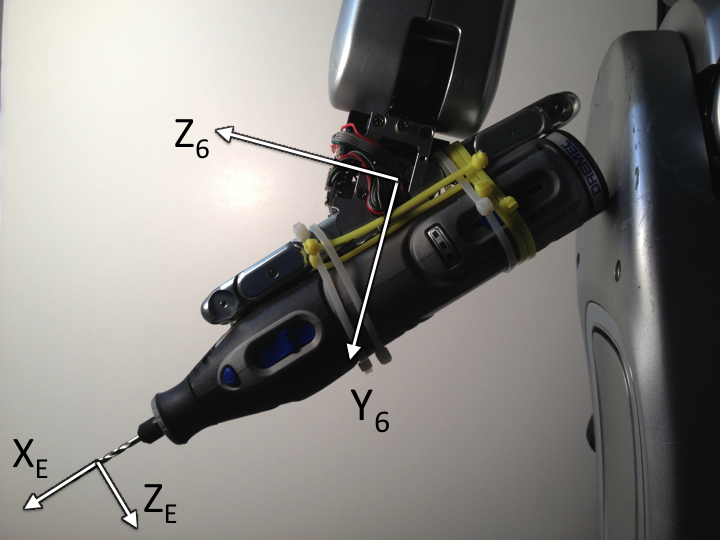
\includegraphics[width=0.3\textwidth]{figures/Drill-Coordinates}
  \caption{Drill end-effector coordinate frames}
  \label{fig:drillCoordinates}
\end{figure}

To find this optimal distance simulations were performed to map the workspace of the end-effector. The results of these simulations are shown in \cref{fig:eeWorkspace}. It was found that a distance of 484 mm from the neck to the wall gives the largest horizontal workspace at 390 mm. This is at a vertical distance of 75 mm above the neck coordinate frame. The joint values for the extreme points in the horizontal direction are the following: far right (minimum y value) $q = [-0.9914, -0.3651, -0.8339, -1.1618, -1.6542, 0.8894]$ and the far left (maximum y value) $q = [-1.1853, 0.1213, 1.1383, -1.2893, -1.8826, -1.1184]$.

\begin{figure}[h]
  \centering
  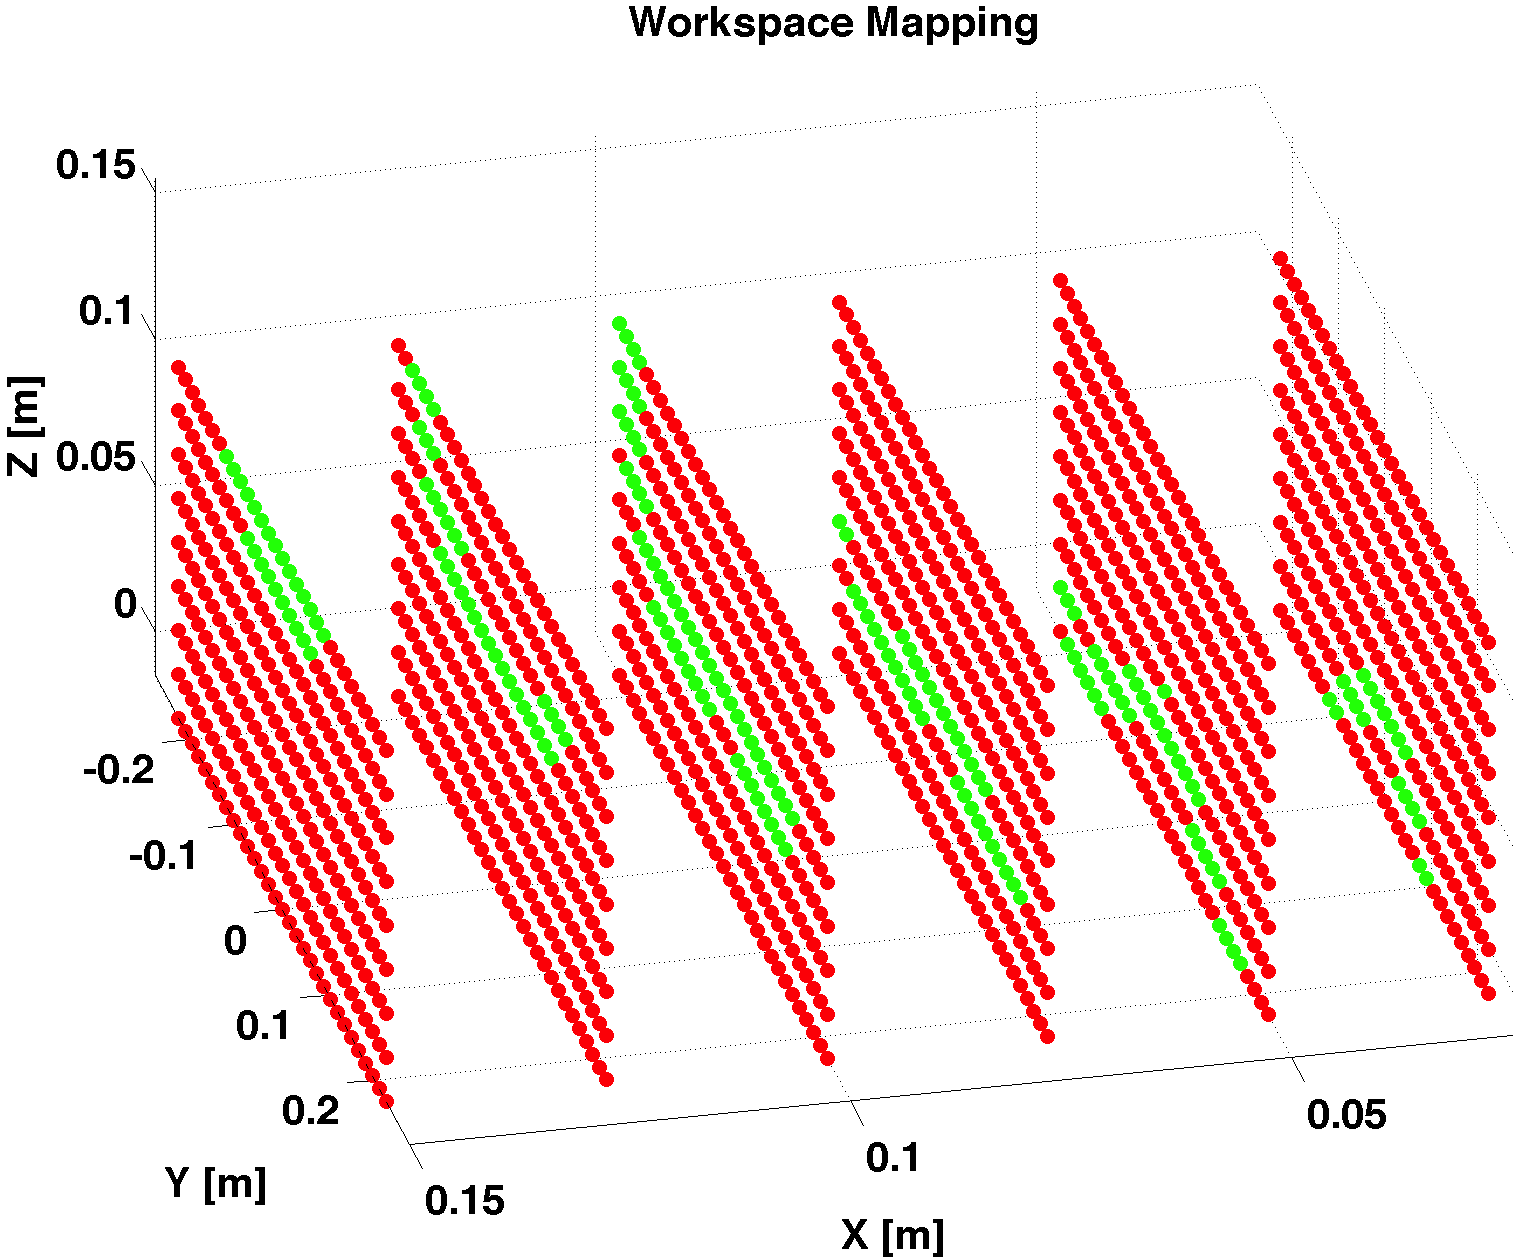
\includegraphics[width=0.35\textwidth]{figures/eeWorkspace}
  \caption{Workspace of the drill bit as the end-effector in reference to the neck coordinate frame. The green points are points that the drill bit can reach and red points are points that the drill bit can not reach if it maintains an orientation such that the bit is orthogonal to the wall. }
  \label{fig:eeWorkspace}
\end{figure}

The orientation of the drill is set to have the drill bit orthogonal to the wall. In addition, the distance from the wall is also set to give the maximum horizontal workspace. Therefore, using teleoperation via FASTRAK to control the orientation and the distance in the x-direction is not possible. The teleoperation in this case only defines the displacement in the y-direction and the z-direction.

In this experiment the wall is made from cardboard and is set 48 cm in front of Hubo. A human operator controlling Hubo via FASTRAK cuts a rectangular hole in the cardboard wall. Both the input from the human is recorded as well as the actual end-effector location. The results are discussed in the next section.

% -------------------------------------------------------------------------------------
% MAIN RESULTS
% -------------------------------------------------------------------------------------
\section{Main Results} \label{sec:mainResults}
In \cref{fig:fastTrakVsEE} we show the results of the teleoperation via FASTRAK to control Hubo to cut a rectangular hole (approximately 15 cm by 10 cm) in a cardboard wall. The figure compares the input trajectory (dashed red line) with the actual trajectory (solid blue line). The cut started in the upper left hand corner and moved around in the counter-clockwise direction. \footnote{Further results and videos of Hubo experiments can be found at http://www.golems.org/projects/hubo.html.}

There is very little variation between the commanded motion and the actual cut in the cardboard. The mean root squared error between the commanded reference trajectory and the actual trajectory was 17 mm. This value is influenced by various factors, such as the acceleration and velocity limits, which can be adjusted in future for optimization. The cut was not perfectly straight, which is largely due to the operator's error. The actual hole that was cut out is shown in \cref{fig:cardboardHole}. The difference in shape between the actual hole and the plot of the end-effector in \cref{fig:fastTrakVsEE} is due to the fact that the drill bit was not cutting the cardboard at the exact same location of where the end-effector frame is located, which is at the end of the drill bit. This causes the plot to be skewed along one edge.

The average torque along the horizontal and vertical directions of the cut were $0.14\,\pm0.03$ Nm and $0.15\,\pm0.03$ Nm, respectively. The maximum torque along these directions of the cut were $0.23$ Nm and $0.35$ Nm, respectively. These torques are controlled, to a degree, by the operator's hand velocity, by moving at a slow, steady speed. This is necessary because it was determined empirically that the wrist joint has a maximum torque limit of $1.21$ Nm. 

\begin{figure}[h]
  \centering
  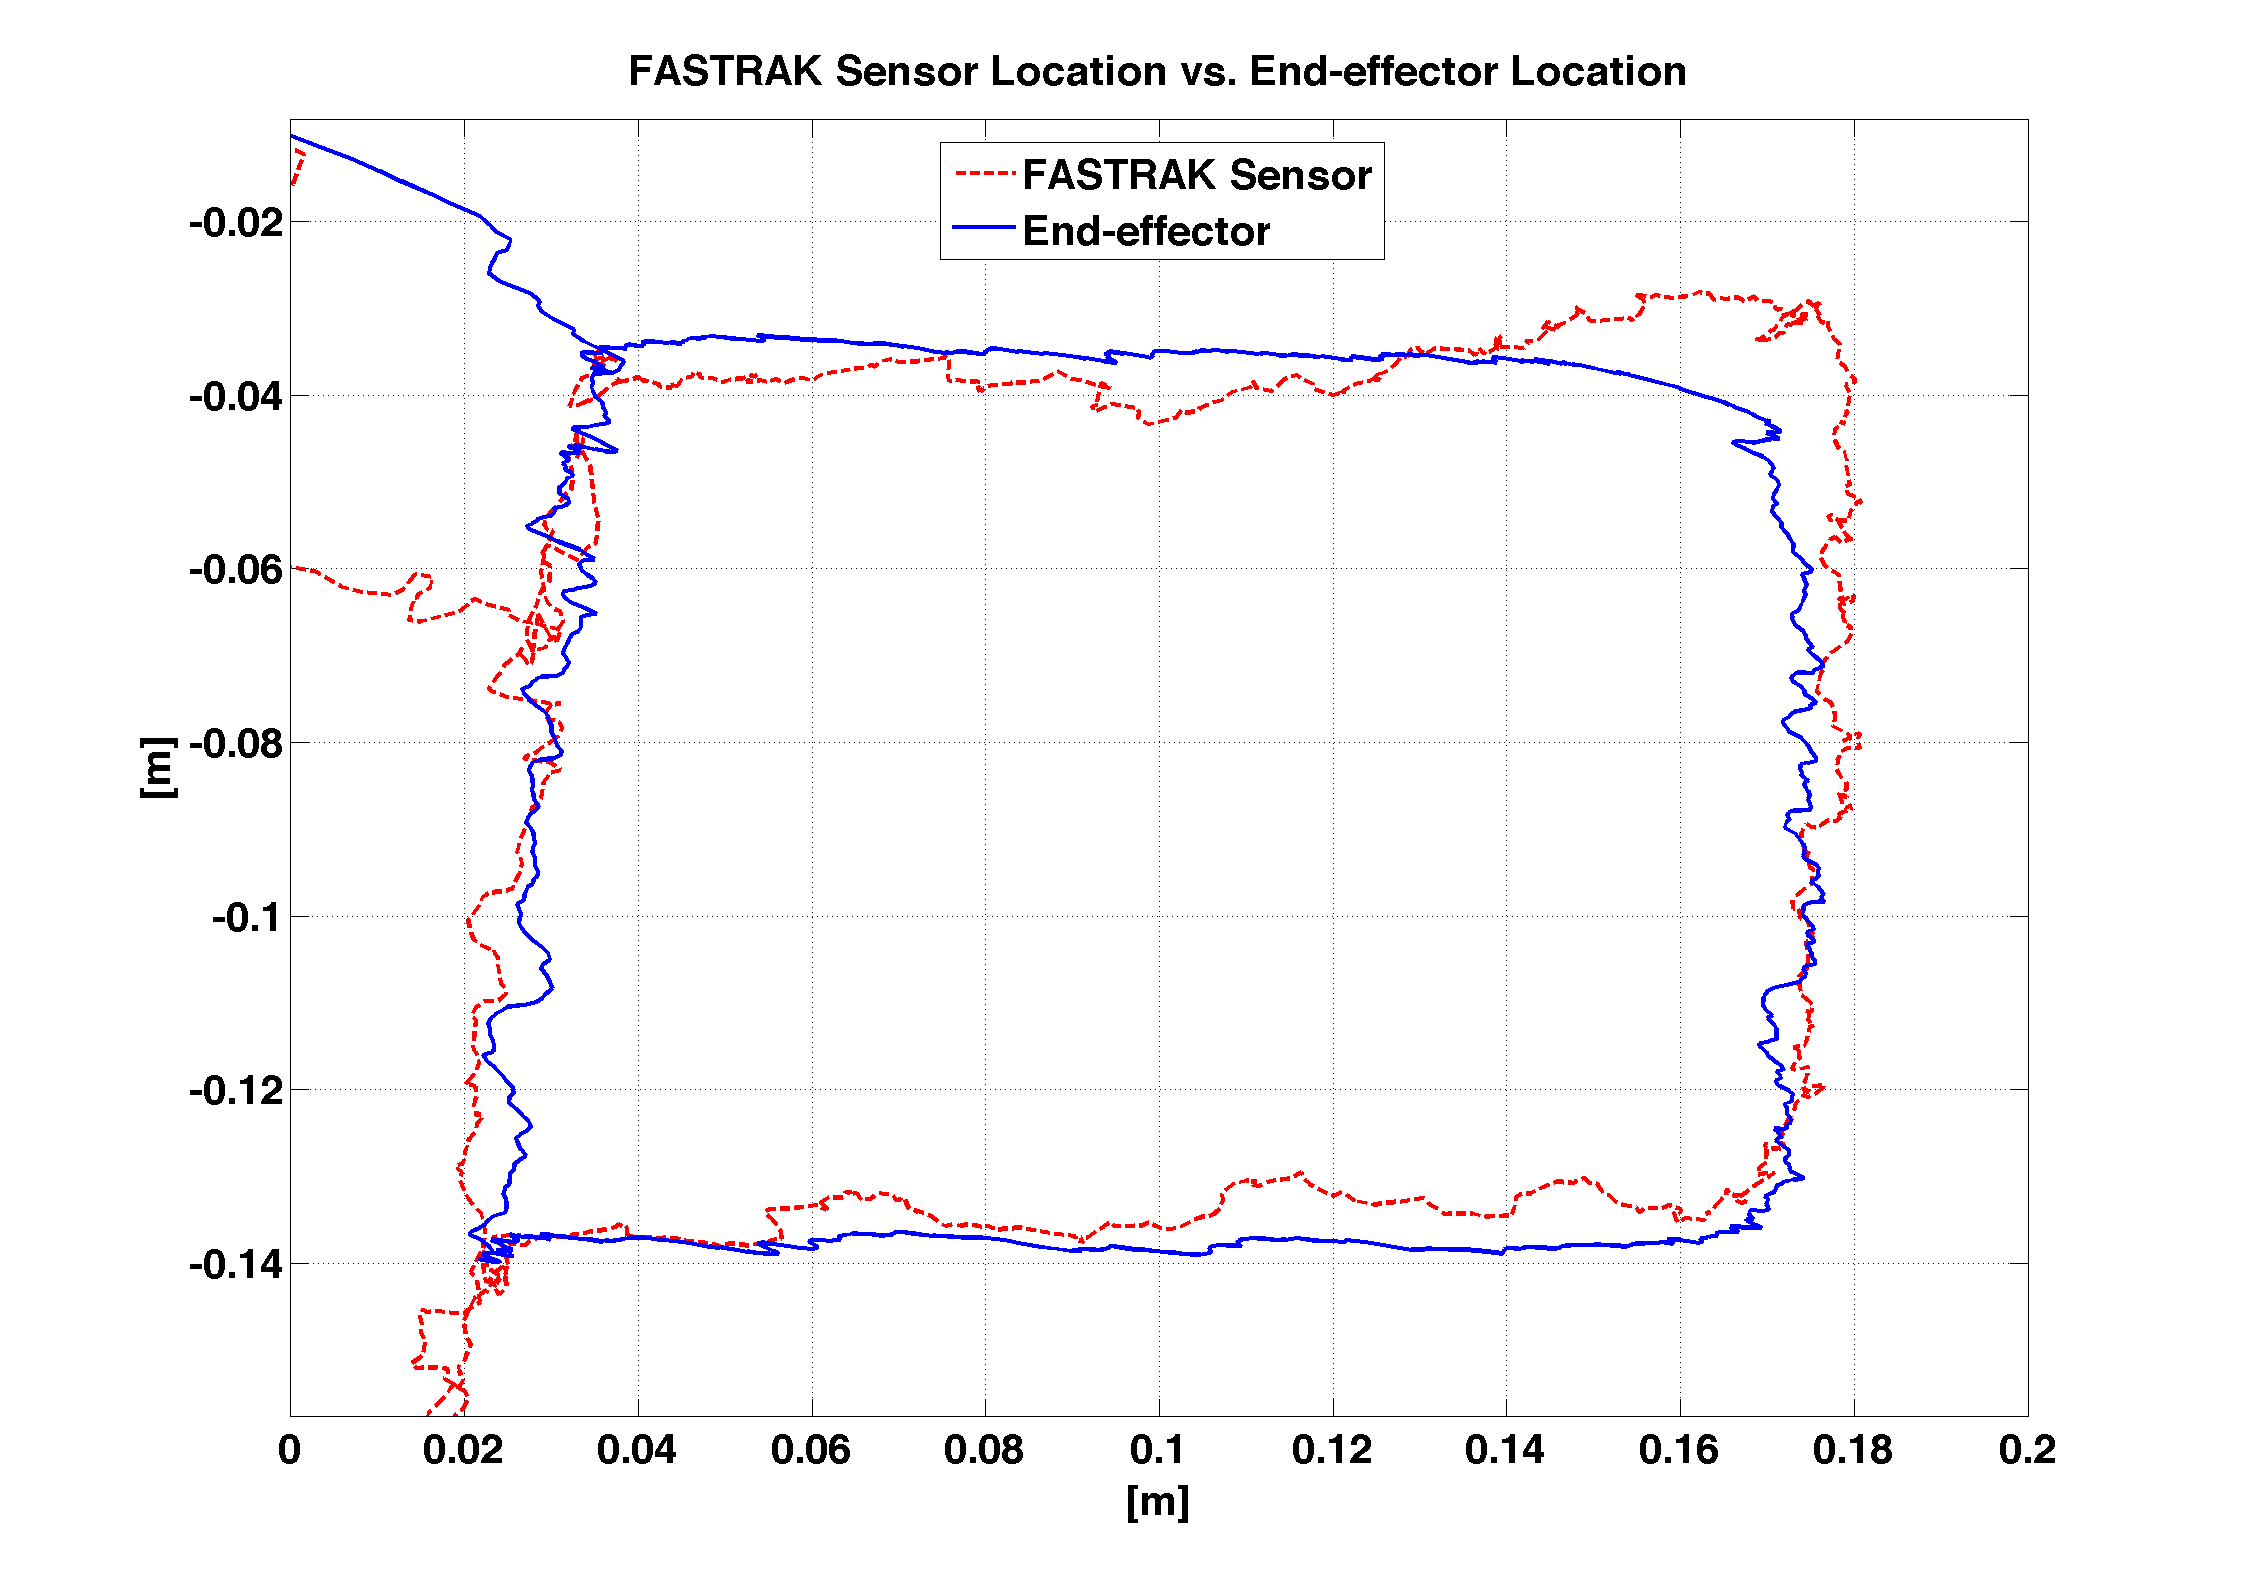
\includegraphics[width=0.39\textwidth]{figures/FASTRAKvsEndEffector}
  \caption{This plot shows a comparison between the user's desired trajectory given via FASTRAK and the actual end-effector location. The dashed red line is the input trajectory and the solid blue line is the actual trajectory.}
  \label{fig:fastTrakVsEE}
\end{figure}

\begin{figure}[t]
  \center
  \subfigure[]{ \label{fig:cardboardHole1}
    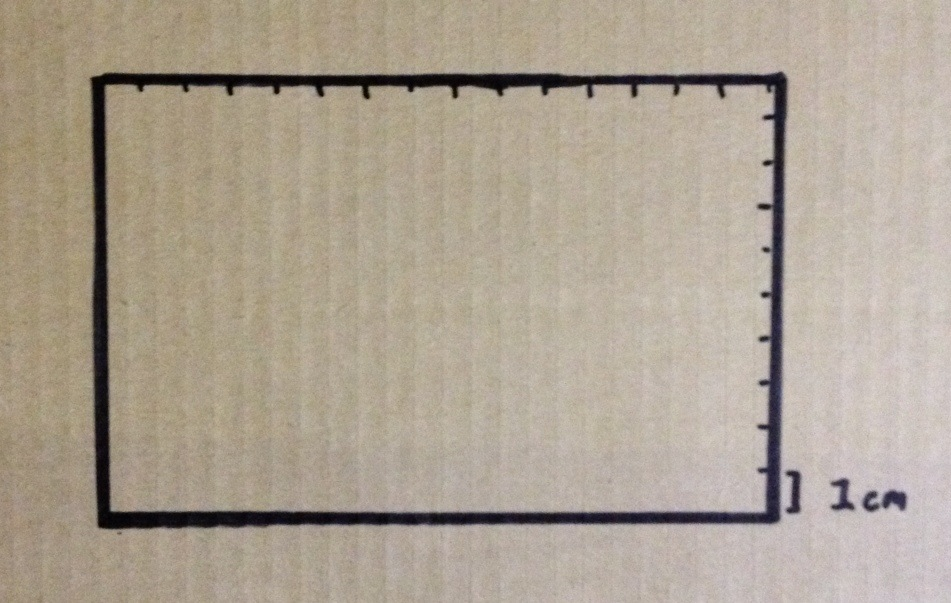
\includegraphics[width=.45\columnwidth]{figures/Hubo-WallCut1}
  }
  \subfigure[]{ \label{fig:cardboardHole2}
    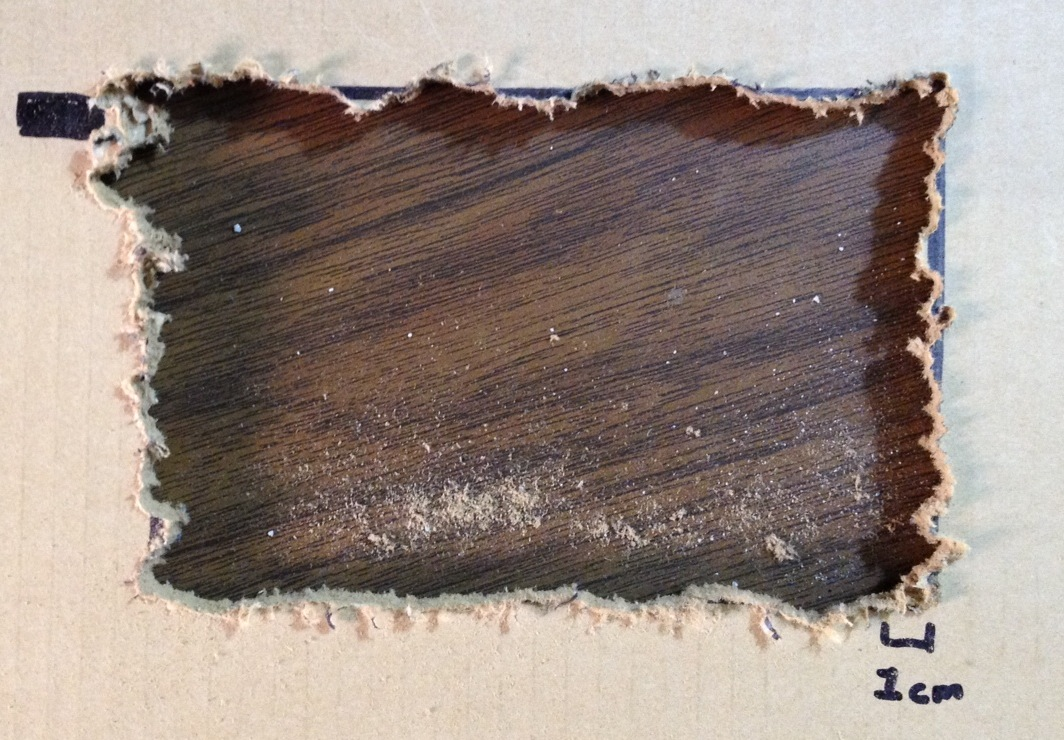
\includegraphics[width=.45\columnwidth]{figures/Hubo-WallCut2}
  }
  \caption{\small Cardboard wall before (a) and after (b) Hubo cutting out a hole via teleoperation.}
  \label{fig:cardboardHole}
\end{figure}

% -------------------------------------------------------------------------------------
% CONCLUSION
% -------------------------------------------------------------------------------------
\section{Conclusion} \label{sec:conclusionAndFutureWork}
In conclusion, we have demonstrated that the HUBO\,2+ humanoid robot is capable of doing tasks that involve manual labor or require power tools. These tasks were performed with teleoperation, but in future work we aim to automate this process by incorporating exteroceptive perceptual feedback and motion planning.

% -------------------------------------------------------------------------------------
% ACKNOWLEDGEMENTS
% -------------------------------------------------------------------------------------
\section{Acknowledgements}
This work was supported in part by DARPA \#N65236-12-1-1005: DARPA Robotics Challenge and NSF CNS-0960061 MRI-R2: Unifying Humanoids Research.

% -------------------------------------------------------------------------------------
% REFERENCES
% -------------------------------------------------------------------------------------
\bibliography{hubo-teleopTasks}

% -------------------------------------------------------------------------------------
% END DOCUMENT
% -------------------------------------------------------------------------------------
\end{document}
